\documentclass{beamer}
\usetheme{metropolis}
\usepackage{graphicx}
\usepackage{subfig}
\title{Safe Return Doubtful: Week 8}
\date{\today}
\author{Jordan Hanson}
\institute{Whittier College Department of Physics and Astronomy}

\begin{document}
\maketitle

\section{Summary}

\begin{frame}{Summary}
\textbf{Astrophysics and cosmology} in Antarctica
\begin{enumerate}
\item South Pole Telescope - SPT
\item BICEP2
\end{enumerate}
What do these experiments do?  What measurements do they make?
\begin{enumerate}
\item The Big Bang
\item Cosmic Microwave Background (CMB)
\end{enumerate}
\end{frame}

\section{The Big Bang}

\begin{frame}{The Big Bang}
\begin{figure}
\centering
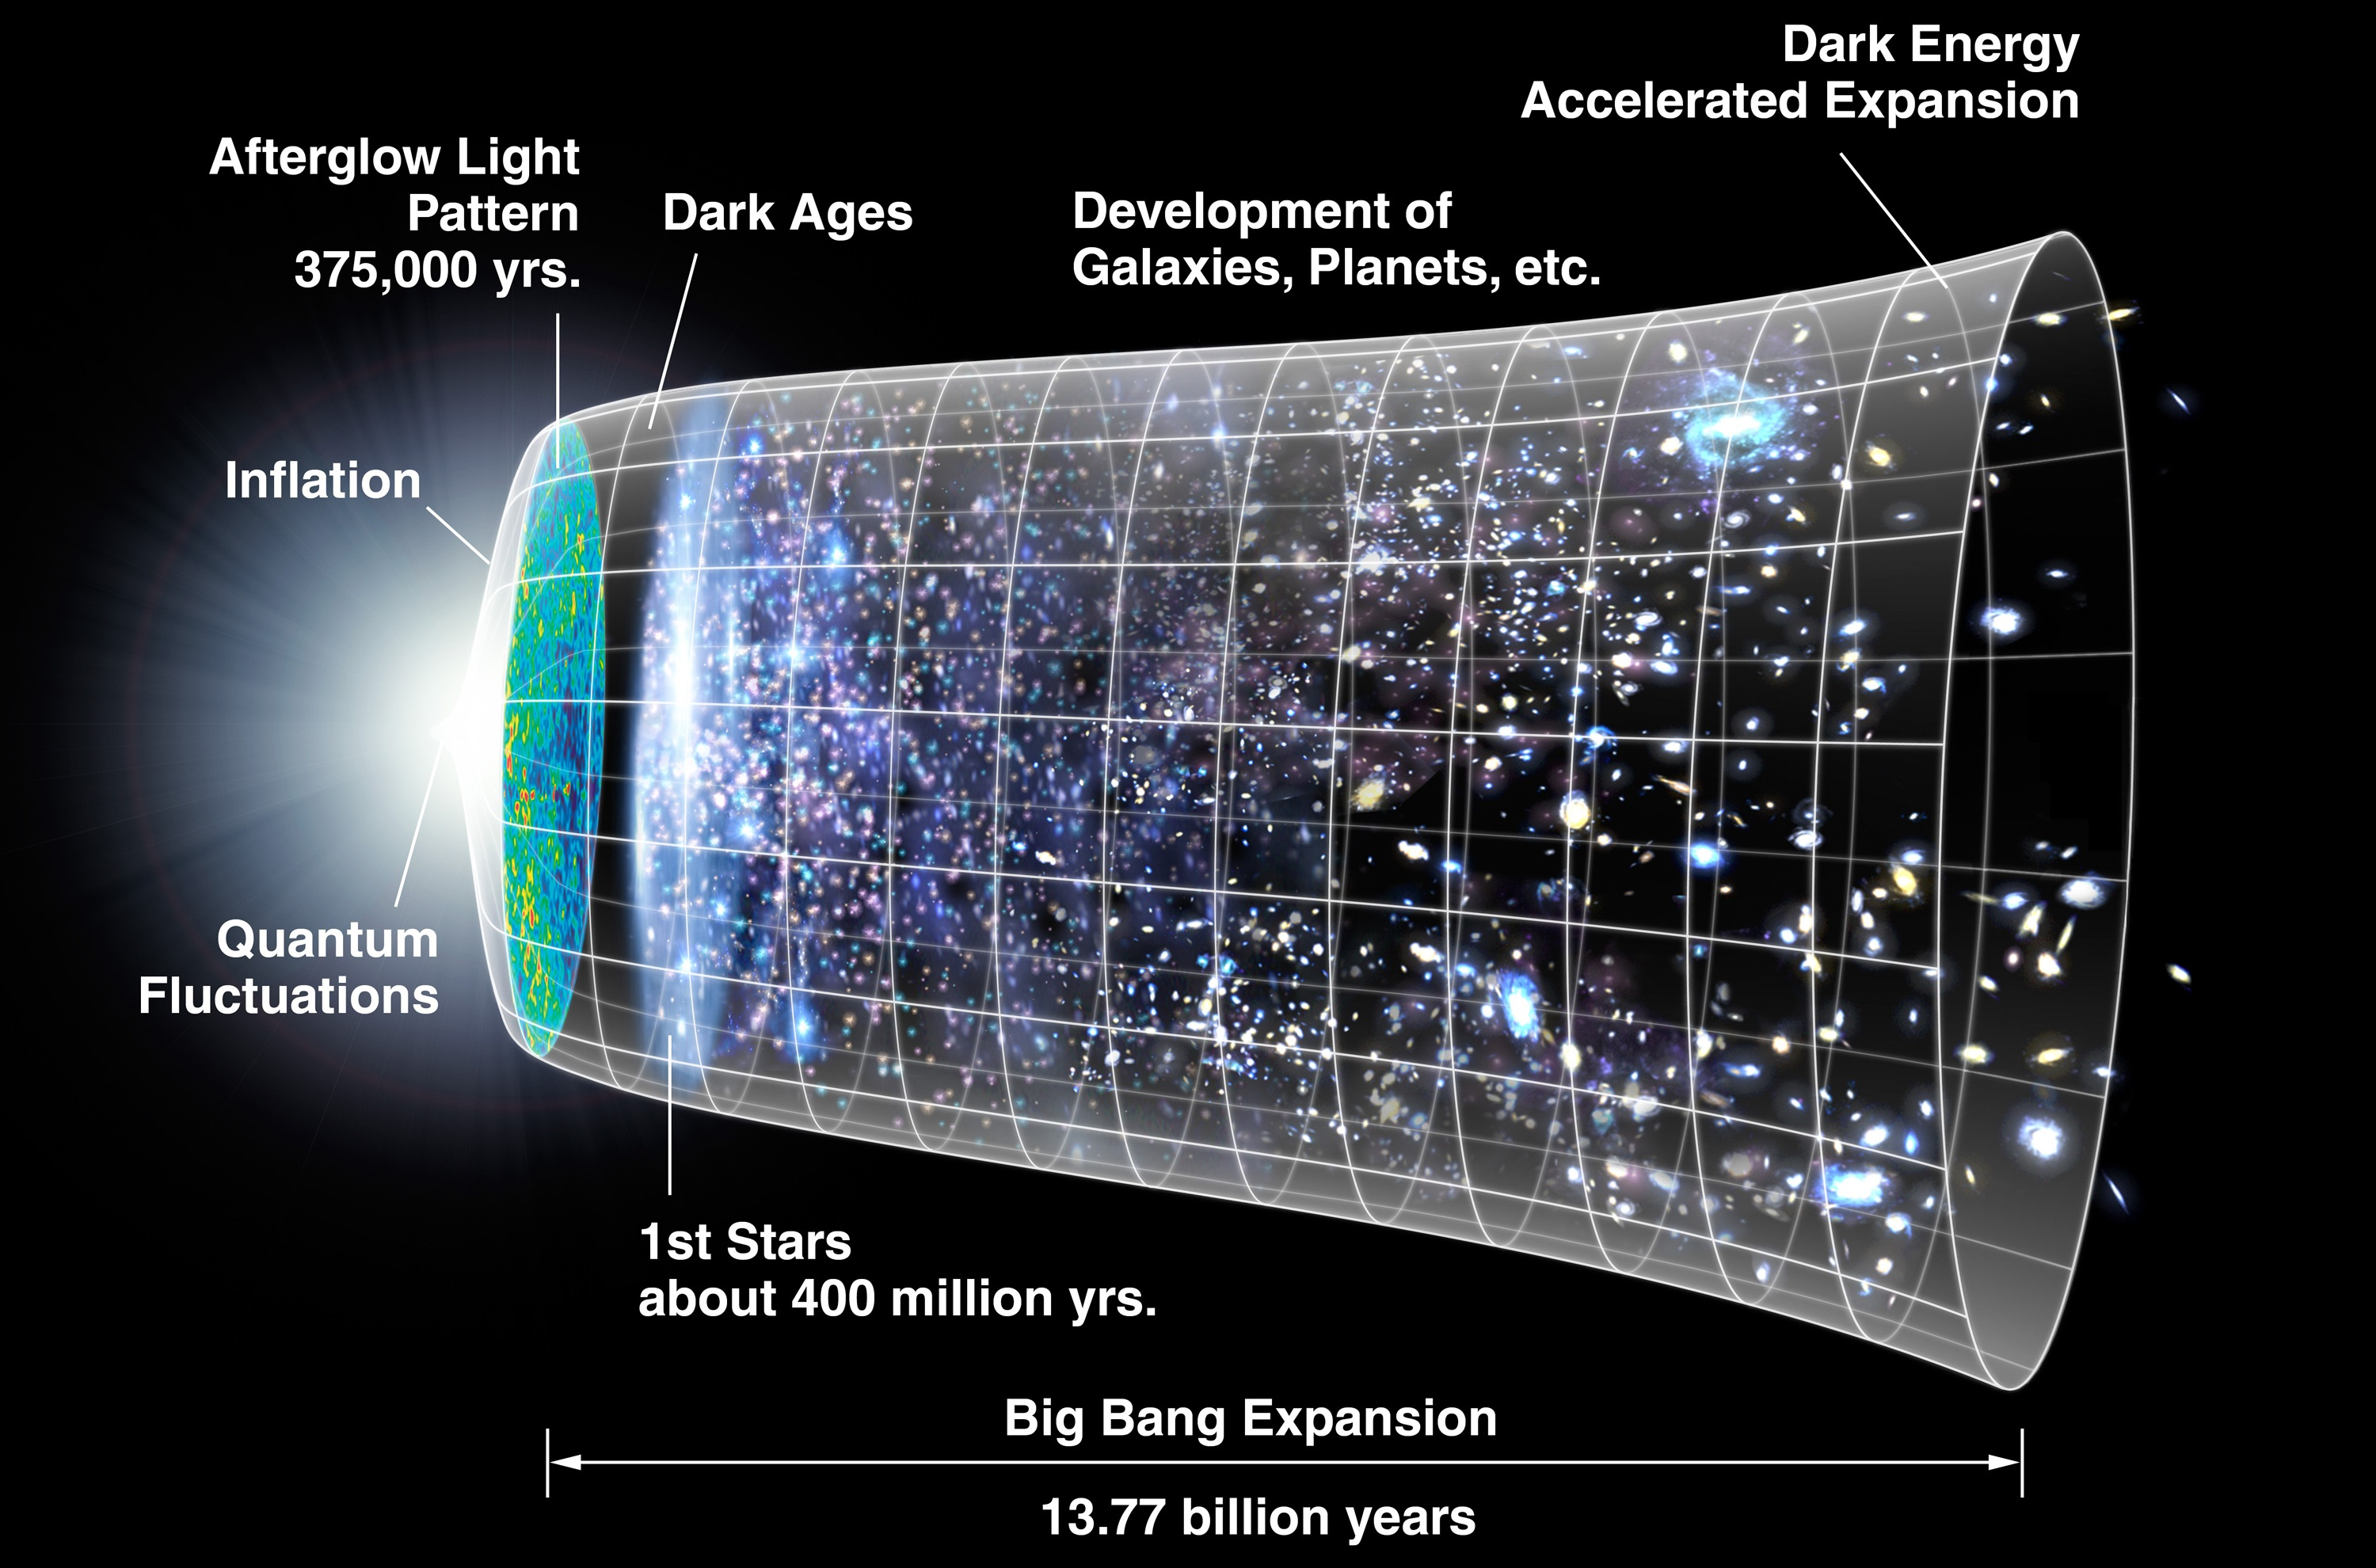
\includegraphics[width=0.75\textwidth]{CMB.jpg}
\caption{\label{fig:cmb} The timeline of the big bang theory and the data behind it.}
\end{figure}
\end{frame}

\begin{frame}{The Big Bang}
\textbf{The Hubble–Lema\^itre law} is the observation in physical cosmology that:
\begin{enumerate}
\item Objects observed in deep space—extragalactic space, 10 megaparsecs (Mpc) or more—are found to have a redshift, interpreted as a relative velocity away from Earth.
\item This Doppler shift-measured velocity of various galaxies receding from the Earth is approximately \textit{proportional} to their distance from the Earth for galaxies up to a few hundred megaparsecs away.
\end{enumerate}
\end{frame}

\begin{frame}{The Big Bang}
What is a Doppler shift?
\begin{enumerate}
\item The pitch of a car horn or ambulance goes \textit{down} as the vehicle recedes from our ears.
\item The wavelength of light does the same thing.
\item The wavelength stretching means the light gets \textit{more red} as objects in space recede from the Earth.
\end{enumerate}
\end{frame}

\begin{frame}{The Big Bang}
\begin{figure}
\centering
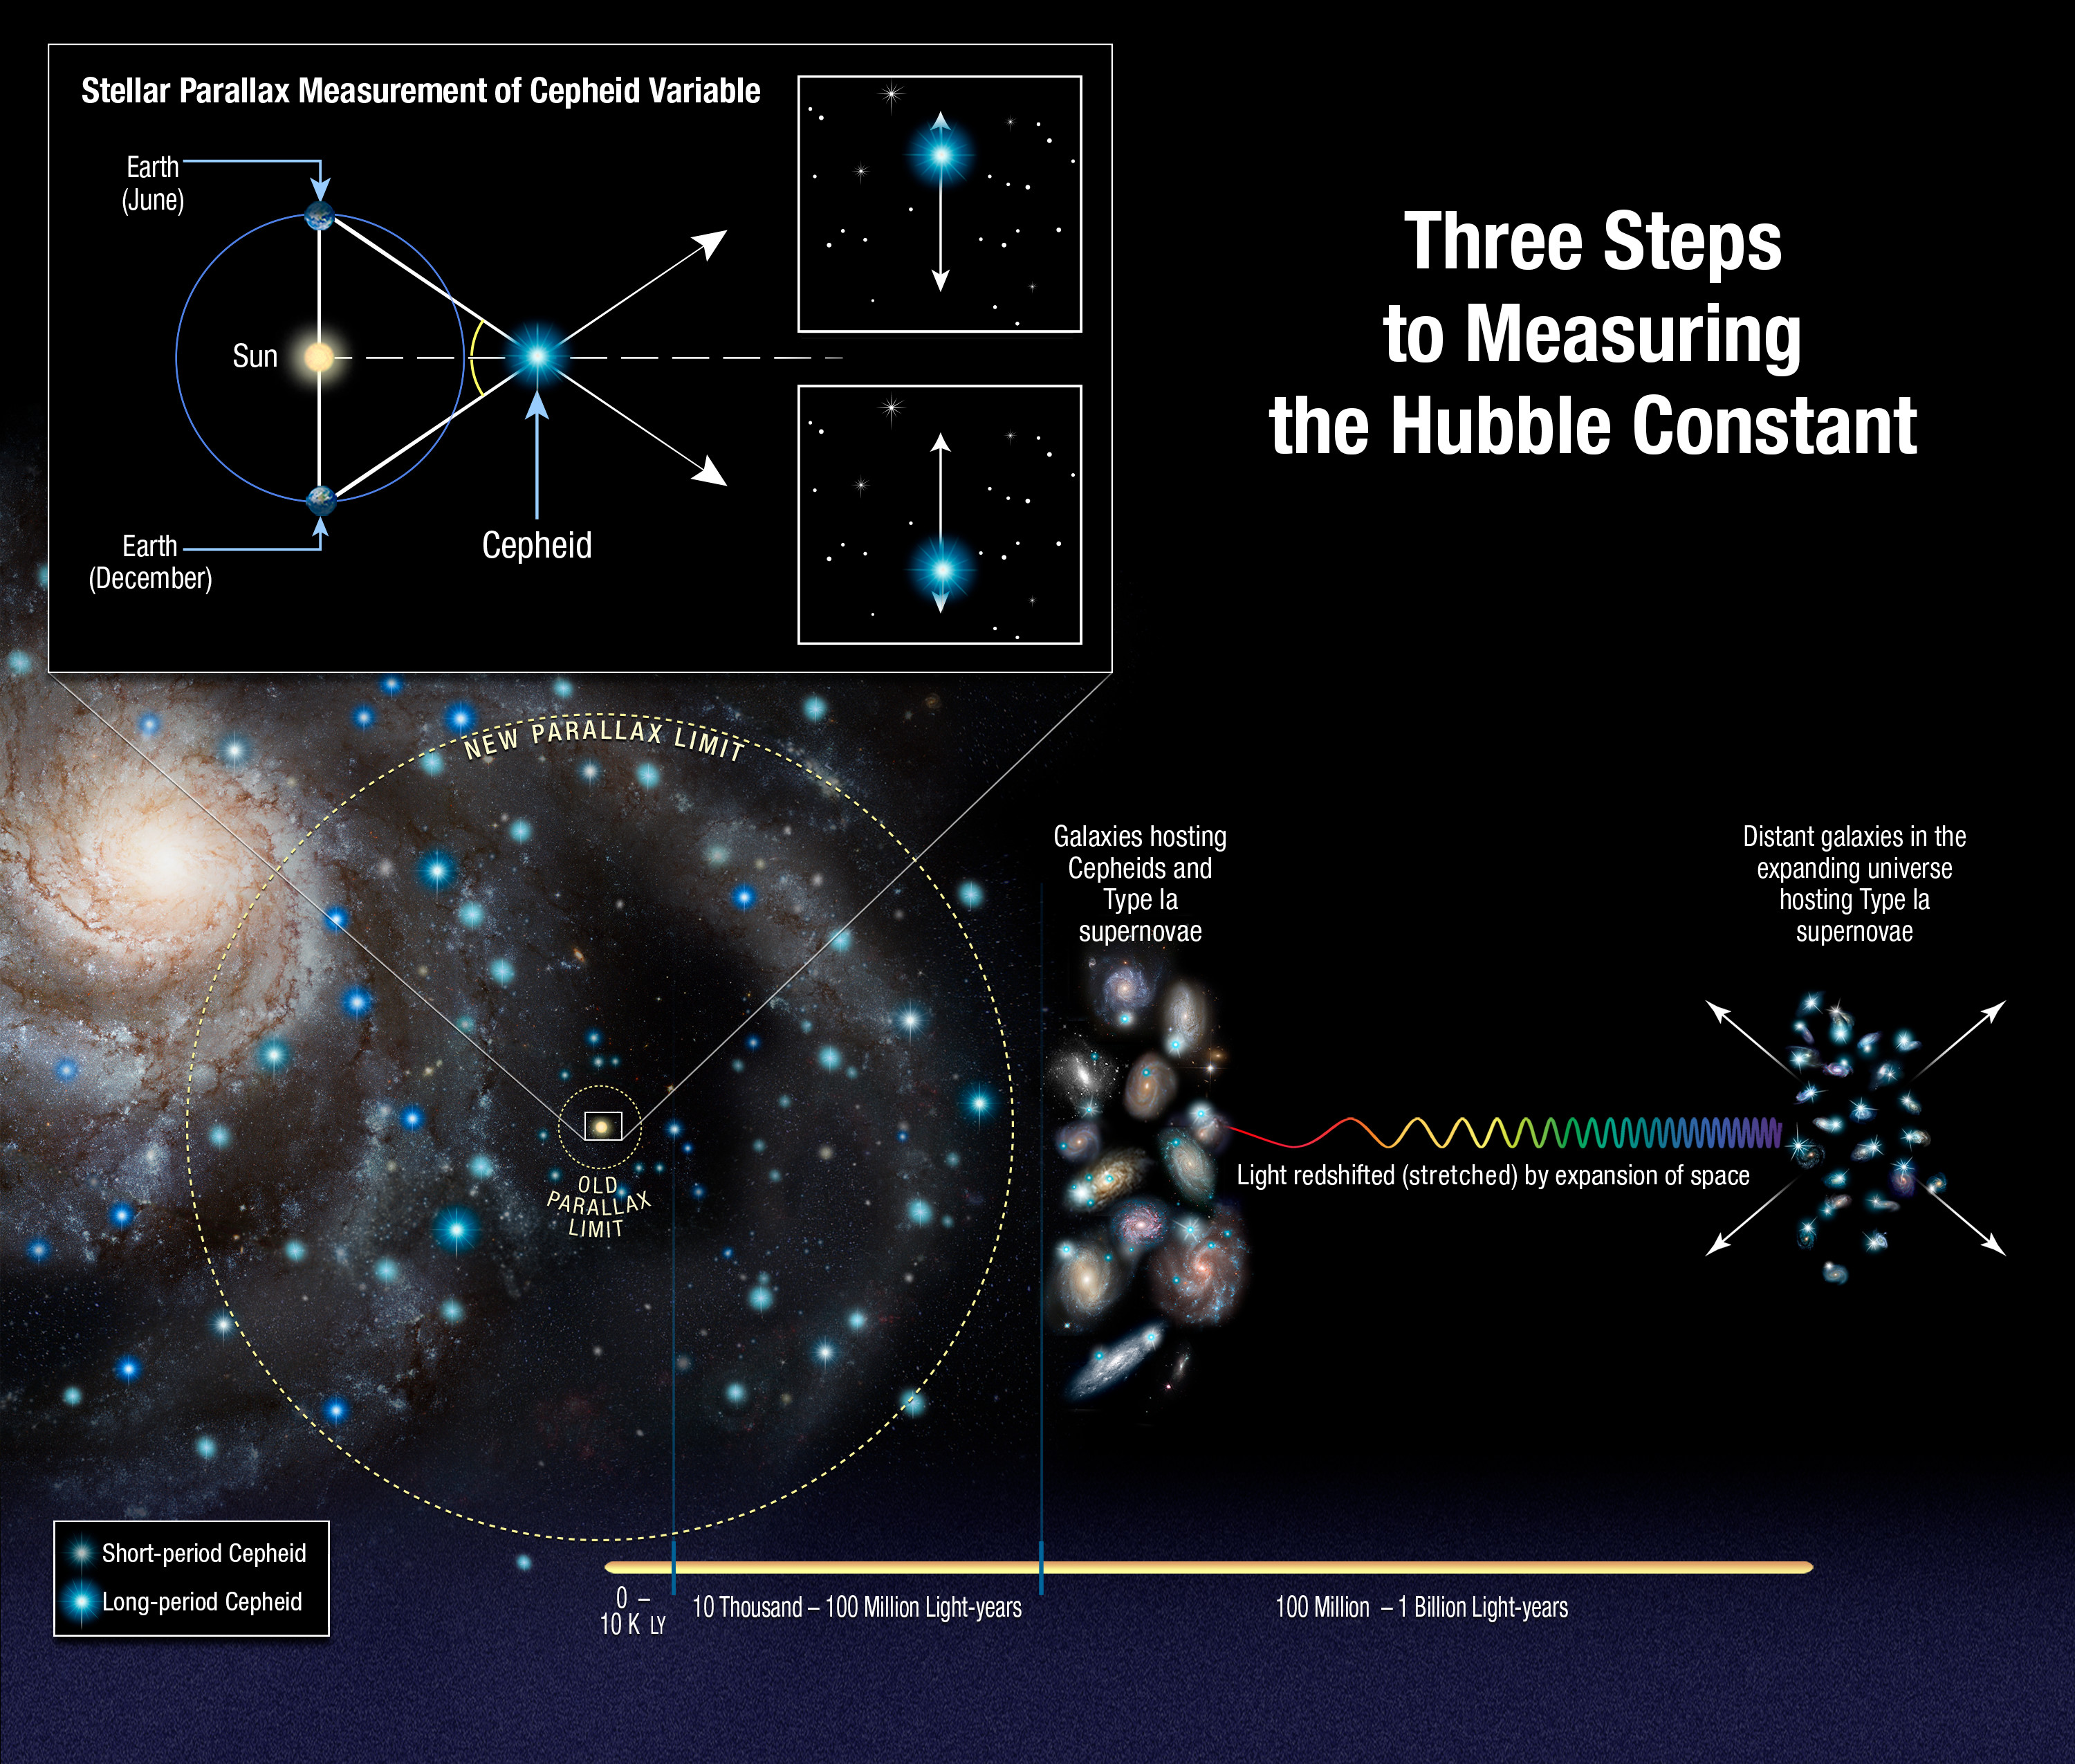
\includegraphics[width=0.65\textwidth]{threesteps.jpg}
\caption{\label{fig:dropin} Edwin Hubble and others characterized the Doppler shift of variable stars in other galaxies, thereby establishing distance and redshift together.}
\end{figure}
\end{frame}

\begin{frame}{The Big Bang}
\begin{figure}
\centering
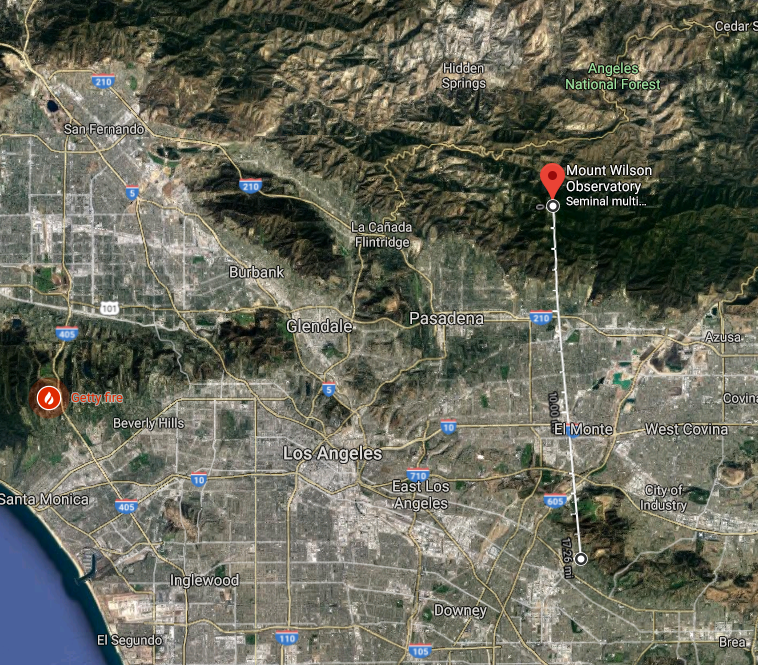
\includegraphics[width=0.65\textwidth]{mountwilson.png}
\caption{\label{fig:cmb3} Mount Wilson Observatory, where Edwin Hubble made many of his famous measurements of cepheid variables in what turned out to be other galaxies.}
\end{figure}
\end{frame}

\begin{frame}{The Big Bang}
\begin{figure}
\centering
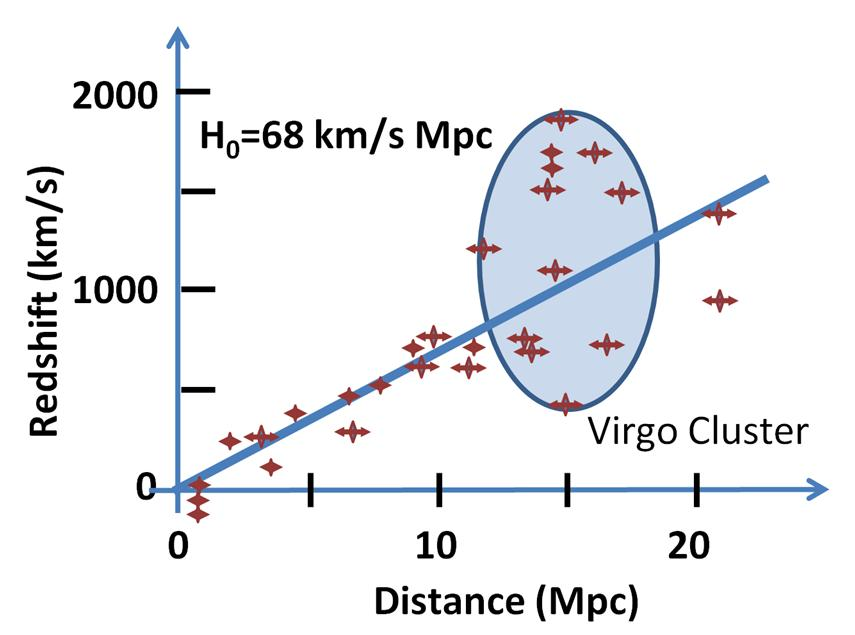
\includegraphics[width=0.75\textwidth]{hubbleConstant.jpg}
\caption{\label{fig:cmb4} Hubble constant fit.  It gives a velocity at a given distance.}
\end{figure}
\end{frame}

\begin{frame}{The Big Bang}
Demonstration: I need some volunteers!
\begin{enumerate}
\item Let's arrange ourselves in a line, holding hands with our hands at our sides.
\item Now, rearrange so that we are still holding hands, but our arms are outstretched.
\item How quickly do the people in the middle have to move?
\item Compare to how quickly the people at the edge must move.
\end{enumerate}
\end{frame}

\section{The Cosmic Microwave Background (CMB)}

\begin{frame}{The Cosmic Microwave Background (CMB)}
\begin{figure}
\centering
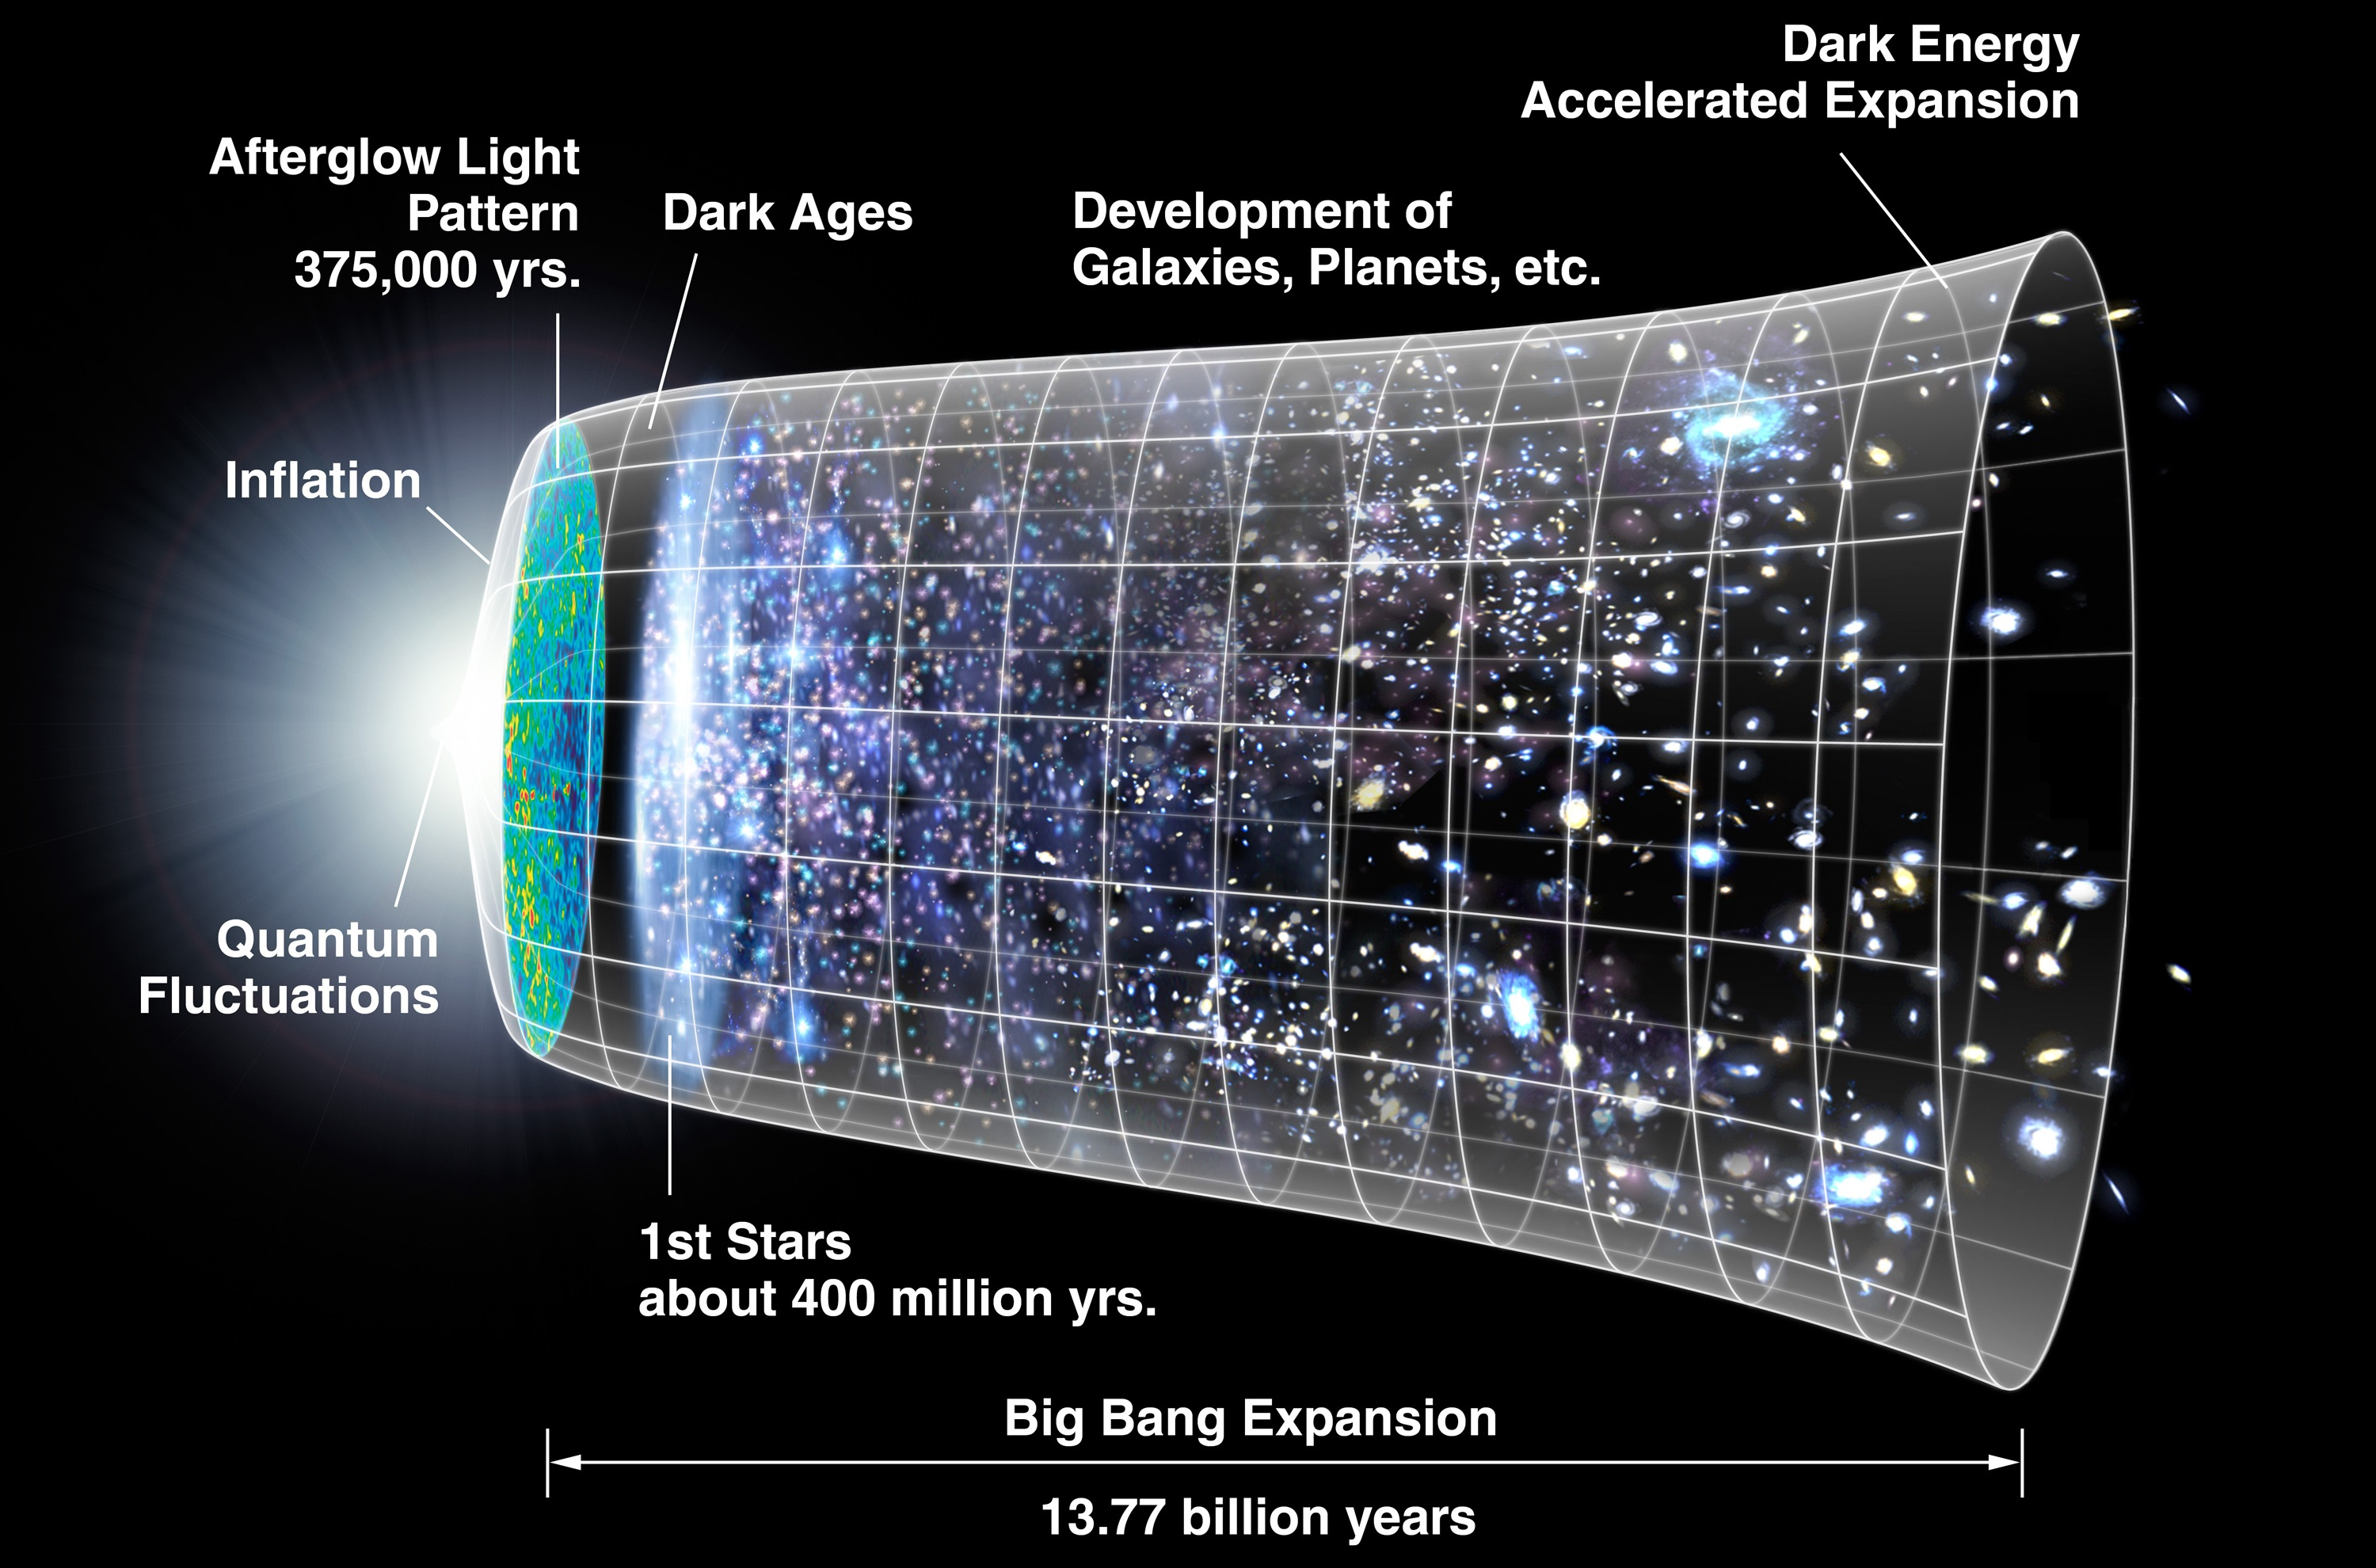
\includegraphics[width=0.75\textwidth]{CMB.jpg}
\caption{\label{fig:cmb5} The beginning of this story is that the universe had certain measurable properties.}
\end{figure}
\end{frame}

\begin{frame}{The Cosmic Microwave Background (CMB)}
\begin{figure}
\centering
\includegraphics[width=0.75\textwidth]{cmbmap.png}
\caption{\label{fig:cmb6} The WMAP-9 CMB data.  Fluctuations are on the order of 1 in 100,000.  The shape is predicted to be uniform, and the energy distribution of the photons is also predicted to be a \textbf{black-body spectrum.}}
\end{figure}
\end{frame}

\begin{frame}{The Cosmic Microwave Background (CMB)}
\begin{figure}
\centering
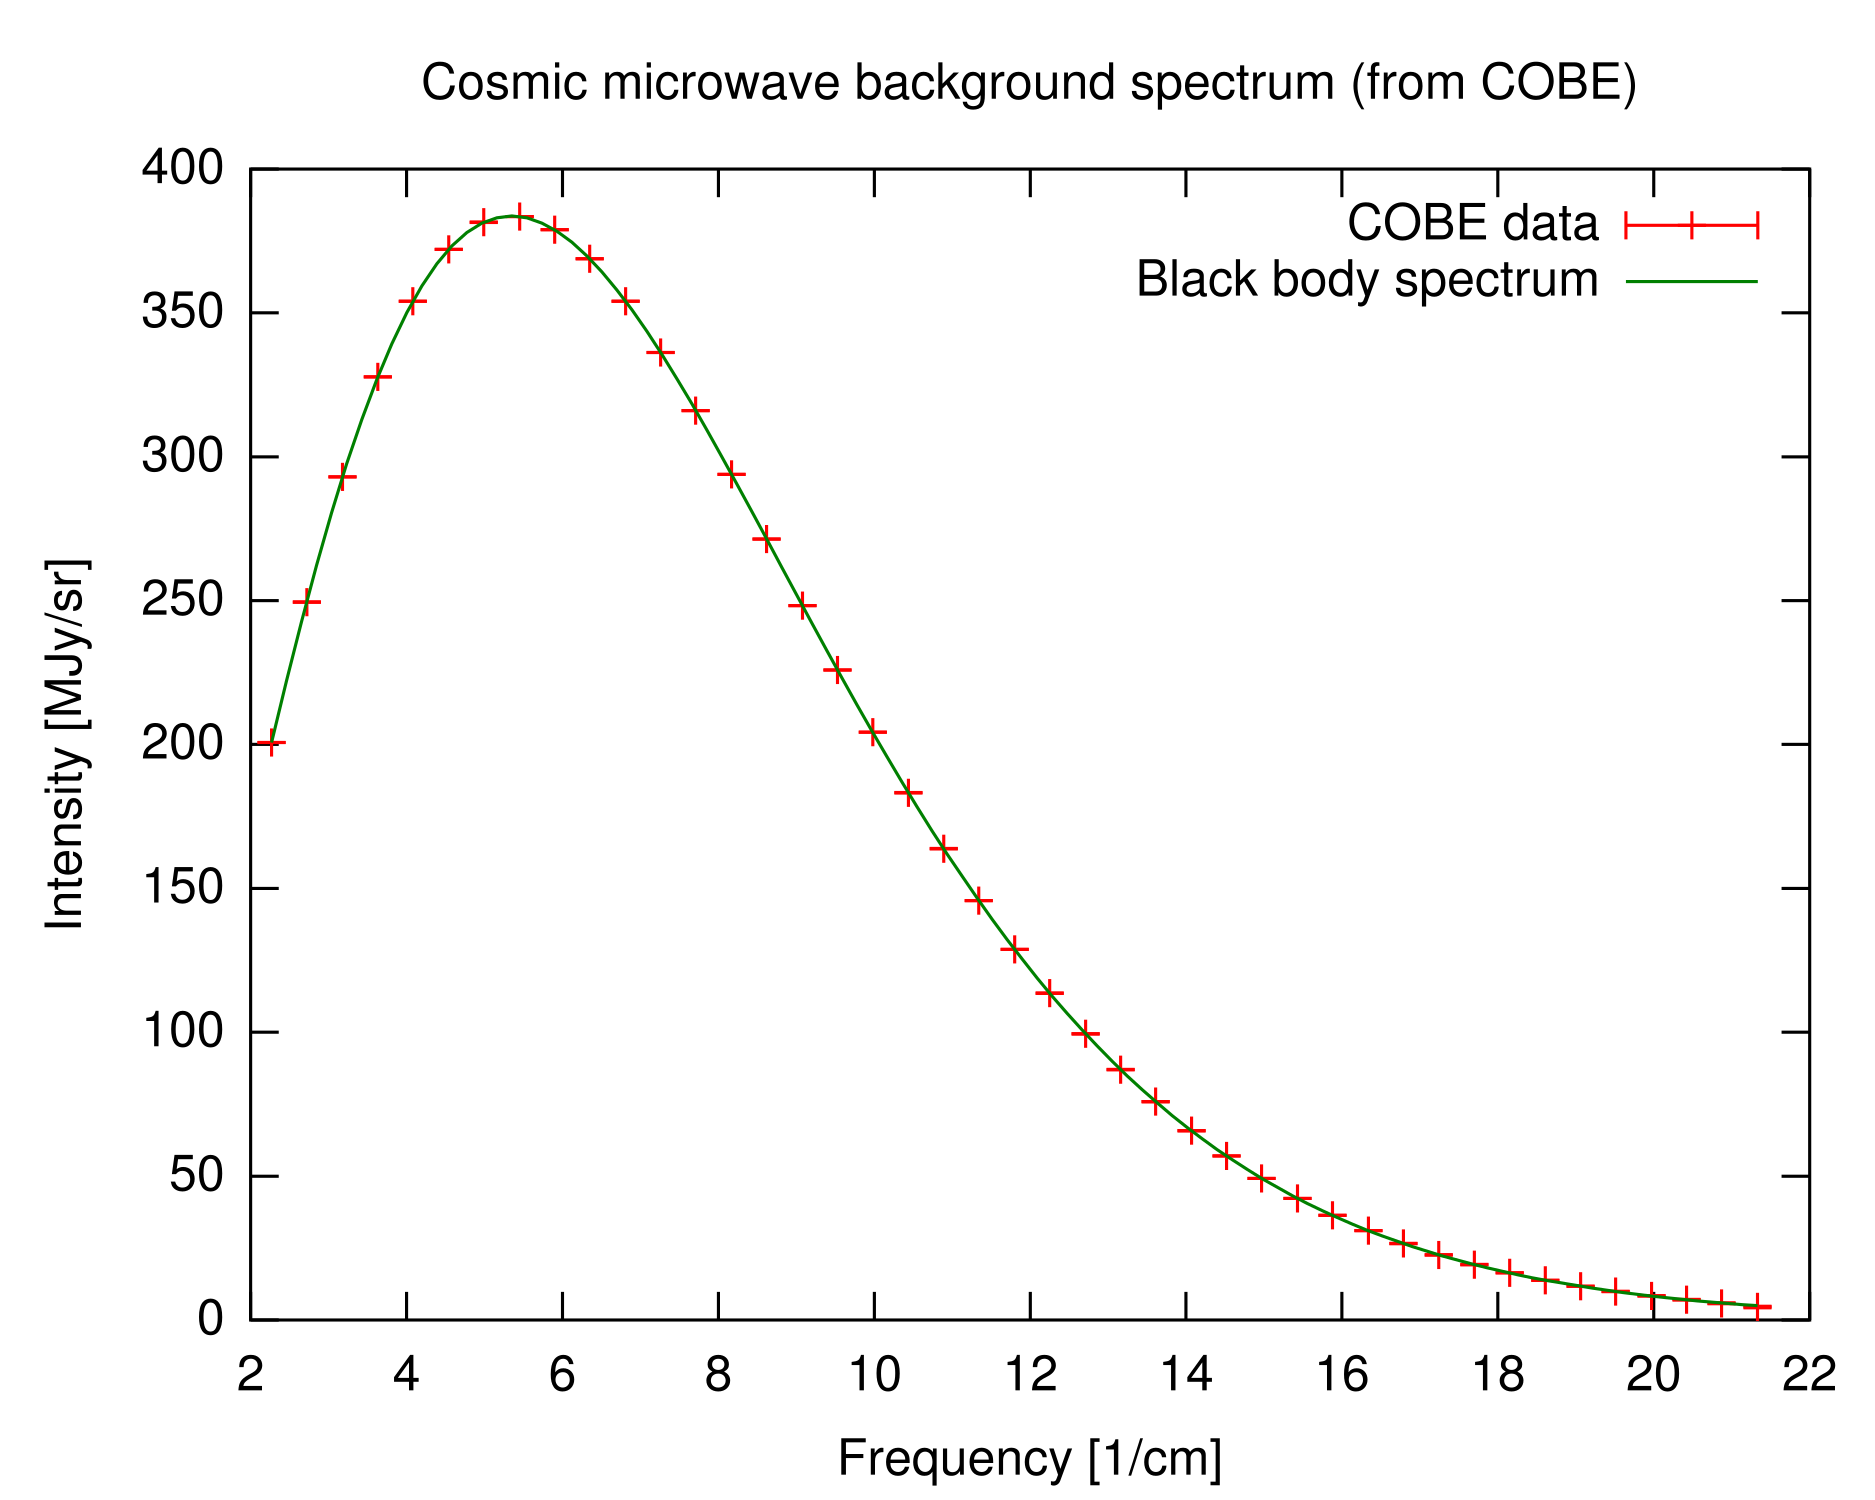
\includegraphics[width=0.75\textwidth]{Cmbr.png}
\caption{\label{fig:cmb7} The measured black-body spectrum from the COBE experiment of the CMB.}
\end{figure}
\end{frame}

\begin{frame}{The Cosmic Microwave Background (CMB)}
\small
How are the modern CMB measurements taken? \\ \vspace{0.25cm}
\url{https://pole.uchicago.edu/public/science.html} \\ \vspace{0.25cm}
\url{https://www.cfa.harvard.edu/CMB/bicep2/science.html}
\end{frame}

\end{document}